\documentclass[./project-report/src/latex/project-report.tex]{subfiles}

\begin{document}

\maketitle

\section{Testing TODO}

\subsection{Investigation}

\subsubsection{test\_model module}

The test\_model module is contained within the frames package, and contains tkinter frames for testing the trained Artificial Neural Network models for each dataset. 
Each frame displays the results of the testing along with a random selection of incorrect and correct predictions.

\inputminted{python}{./school_project/frames/test_model.py}

Which outputs the following for the MNIST dataset:

\pagebreak

\begin{figure}[h!]
\centering
\frame{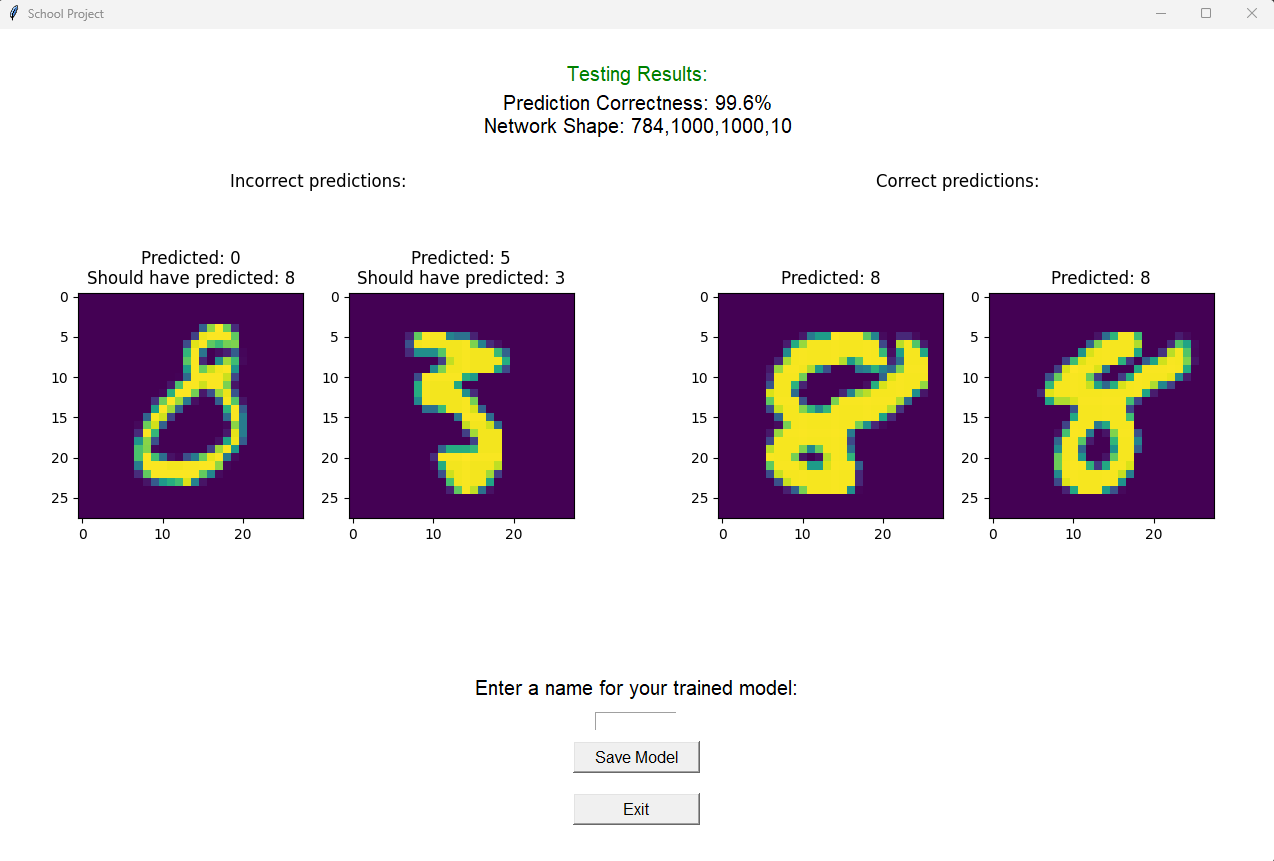
\includegraphics[width=1\textwidth]{./project-report/src/images/test-mnist-frame.png}}
\end{figure}

And outputs the following for the Cat Recognition dataset:

\pagebreak

\begin{figure}[h!]
\centering
\frame{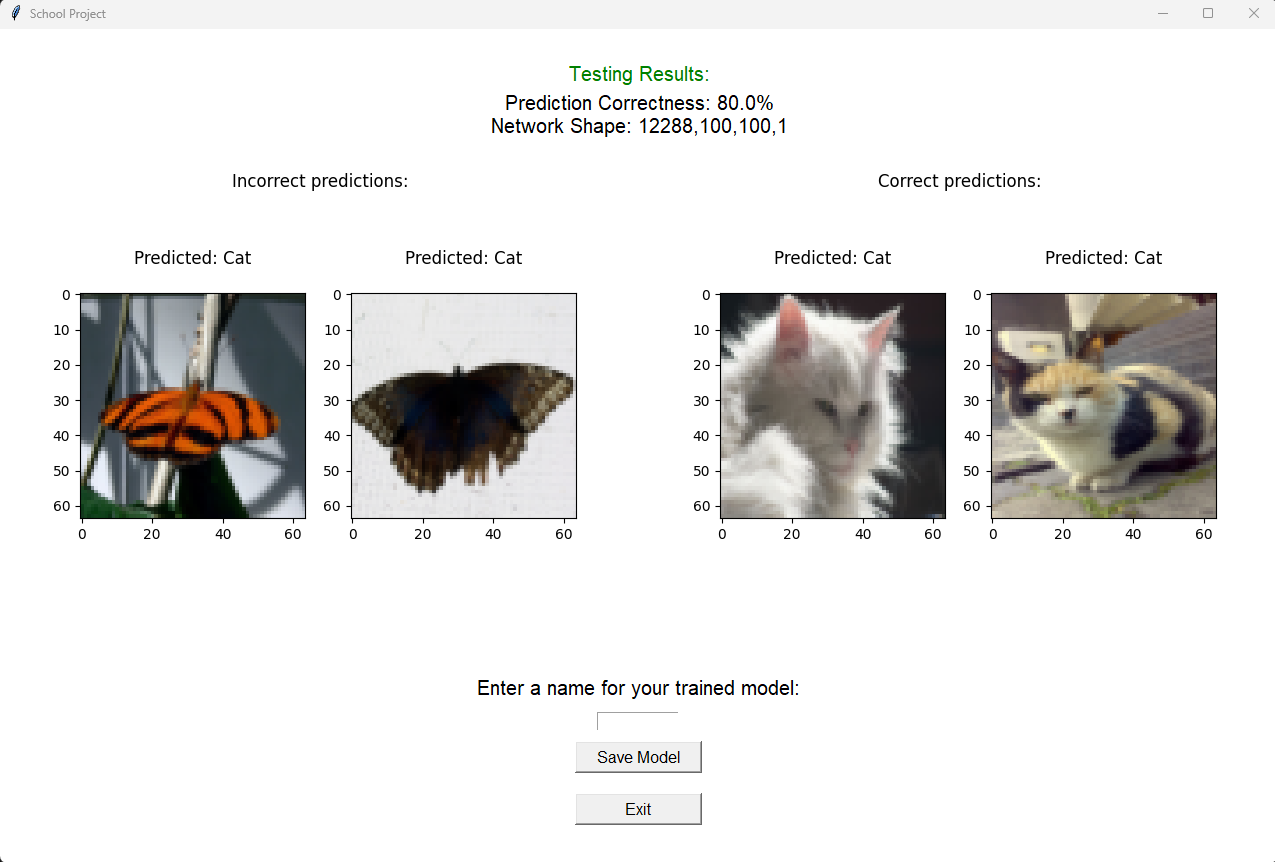
\includegraphics[width=1\textwidth]{./project-report/src/images/test-cat-recognition-frame.png}}
\end{figure}

And outputs the following for the XOR dataset:

\pagebreak

\begin{figure}[h!]
\centering
\frame{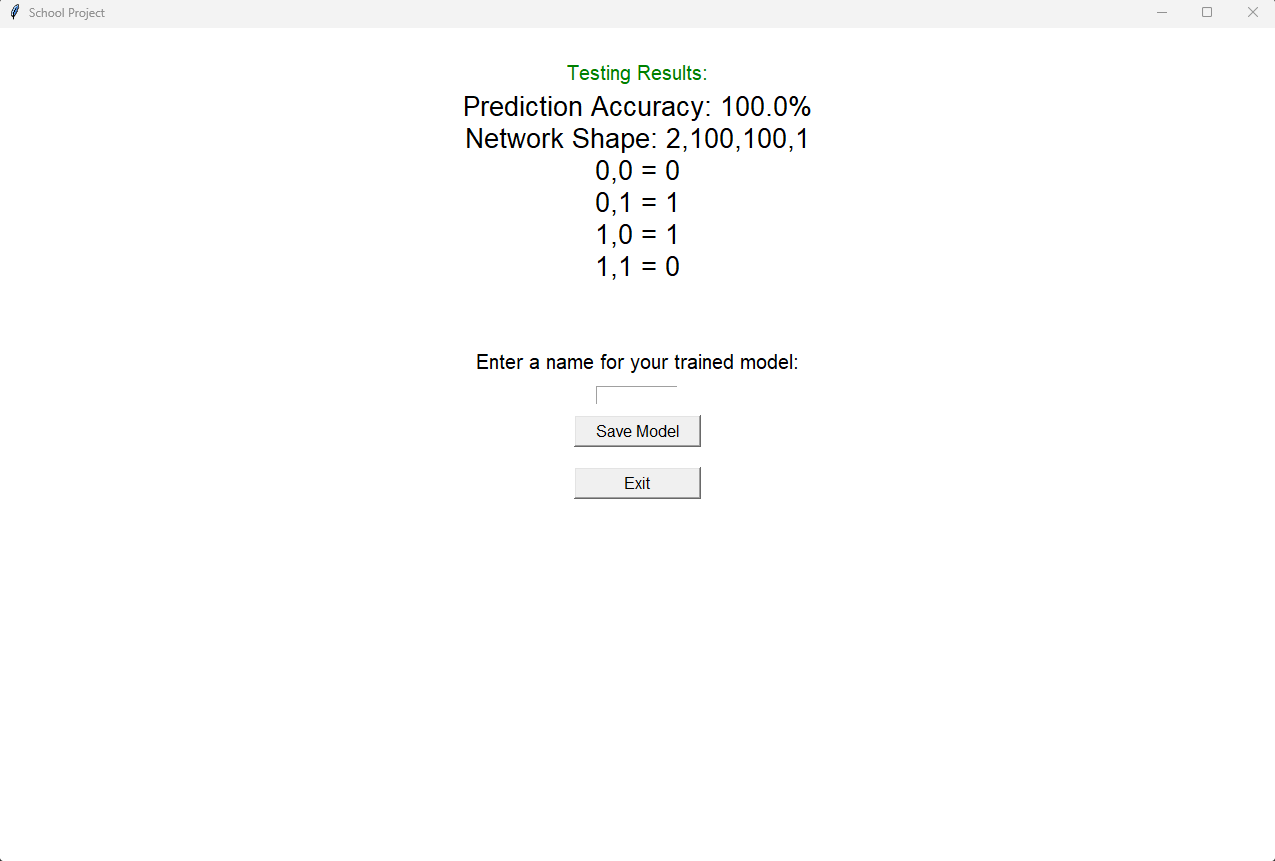
\includegraphics[width=1\textwidth]{./project-report/src/images/test-xor-frame.png}}
\end{figure}

\subsubsection{Effects of Hyper-Parameters}

\subsection{Manual Testing}

\subsubsection{Input Validation Testing}

\subsection{Automated Testing}

\subsubsection{Unit Tests}

\subsubsection{GitHub Automated Testing}

\end{document}